
\chapter{实验中常用的NMR样品及相关实验工作}

目前,实验上常用的NMR样品如表\ref{allsample}所示,而常用的液体溶剂为氘代丙酮(d$_6$-acetone),重水(D$_2$O)以及氘代氯仿(CDCl$_3$),液晶溶剂
则为ZLI-1132。这里仅仅给出了3 qubit以上的NMR样品,且并没有给出单晶NMR样品,下面的说明则会把其余的常用样品一起补上,并给出本实验室利用该样品完成的实验以供参考和查阅。除非特别指明,所有样品的
参数及谱图均是Bruker 400MHz NMR谱仪上的测试结果。

\begin{figure}[htbp]
            \begin{center}
              \includegraphics[width= 0.8\columnwidth]{figures/allsample.pdf}
              \caption{NMR量子计算实验常用的3-10 qubit样品。}
              \label{allsample}
            \end{center}
\end{figure}

\section{2 qubit 液体NMR样品$^{13}$C标记的氯仿(Chloroform)}

作为最常用的,也是最早被应用的2 qubit样品,溶于氘代丙酮中氯仿的分子式为CHCl$_3$,其结构与$^{13}$C的热平衡谱参见图\ref{samplechlorofom}。可以看出,氯仿的谱线非常纯净。其哈密顿量形式为
\begin{eqnarray}
\mathcal{H}_{int}=\omega_1I_z^1+\omega_2I_z^2+2\pi J I_z^1I_z^2.
\end{eqnarray}
$J$耦合常数的大小为214.6Hz,Larmor频率则可以通过设置照射点$O_1$和$O_2$均为0。

\begin{figure}[htbp]
            \begin{center}
              \includegraphics[width= 0.8\columnwidth]{figures/samplechlorofom.pdf}
              \caption{(a)2 qubit 氯仿样品的分子结构,$^{13}$C与$^{1}$H分别用作两个qubit。(b)$^{13}$C的热平衡谱。}
              \label{samplechlorofom}
            \end{center}
\end{figure}

由于两个qubit分别处在C通道和H通道,且NMR谱线也比较纯净,还可以通过H通道去耦转化为1 qubit样品,因此氯仿是低量子位非常有用的样品。我们在该样品上完成的NMR实验有
不利用纠缠解决Bernstein-Vazirani奇偶性问题\cite{app1},量子博弈的实验研究\cite{app2},量子随机行走的实验实现\cite{app3},混态几何相的观测\cite{app4},
Heisenberg自旋链模型中量子相变的观测\cite{app5},近似克隆的实验研究\cite{app6} ,高保真度的几何量子门\cite{app7},完全对称信息的广义测量\cite{app8},哈密顿量对模型的模拟\cite{nmrsim6},$1\rightarrow2$ 的非对称相位不变量子克隆\cite{app9},量子绝热条件充要性的研究\cite{app10},单观测算子测量完整的量子态信息\cite{app11},三能级系统的几何相观测\cite{app12},氢分子能级模拟\cite{static}, 量子退火算法解决旅行商问题\cite{app13}等等。

\section{2 qubit 液晶NMR样品1溴2,3,5氯苯(1-bromo-2,3,5-dichloro-benzene)}

2 qubit的液晶样品1-bromo-2,3,5-dichloro-benzene采用的是苯环上的两个$^{1}$H用作qubit(图\ref{samplelq2}(a)),溶于ZLI-1132。其哈密顿量形式为
\begin{eqnarray}
\mathcal{H}_{int}=\omega_1I_z^1+\omega_2I_z^2+2\pi J I_z^1I_z^2+\pi D(2I_z^1I_z^2-I_x^1I_x^2-I_y^1I_y^2).
\end{eqnarray}
各项参数为$\omega_1/2\pi = 2597.8$Hz,$\omega_2/2\pi = 2508.5$Hz,$D= 434.26$Hz,$J = 2.26$Hz。$J$耦合是通过把样品溶于Acetone中测出的。

\begin{figure}[htbp]
            \begin{center}
              \includegraphics[width= 0.8\columnwidth]{figures/samplelq2.pdf}
              \caption{(a)2 qubit 1-bromo-2,3,5-dichloro-benzene的分子结构,处于不同化学环境的$^{1}$H用作两个qubit。(b)$^1$H的热平衡谱。}
              \label{samplelq2}
            \end{center}
\end{figure}

由于液晶NMR样品哈密顿量的特殊性,该样品并不太适合实现常用的量子计算任务。针对一些特殊形式的量子模拟用哈密顿量,
该样品可能会发挥一定的作用。

\section{3 qubit 液体NMR样品Diethyl-fluoromalonate}

和氯仿一样,这是最常用的3 qubit液体样品,因为其三个qubit分别是三个不同的原子核$^{19}$F, $^{13}$C, 和$^1$H代表,可以把化学位移均通过照射点设置为0,且所有原子核的退相干时间均大于1秒。
其分子结构见图\ref{sampleCHF},其哈密顿量为
\begin{eqnarray}
\mathcal{H}_{int}=\sum\limits_{j=1}^3 {2\pi \nu _j } I_z^j  + \sum\limits_{j < k,=1}^3 {2\pi} J_{jk} I_z^j I_z^k.
\end{eqnarray}

\begin{figure}[htbp]
            \begin{center}
              \includegraphics[width= 0.8\columnwidth]{figures/sampleCHF.pdf}
              \caption{(a)Diethyl-fluoromalonate的分子结构以及系统参数。 椭圆标记的$^{19}$F, $^{13}$C, 和$^1$H核自旋被用作3个qubit。(b)$^{13}$C的热平衡谱。}
              \label{sampleCHF}
            \end{center}
\end{figure}

使用该样品要注意的问题有两点:首先,NMR谱仪要确定有F通道。其次,由于$^{13}$C是未标记的,所以
$^1$H和$^{19}$F的信号都要SWAP到$^{13}$C上进行观测。尽管如此,该样品依旧是最好用的3 qubit液体NMR样品,上面完成的实验有局域与非局域量子态的量子互补性验证\cite{app14},质因数分解21\cite{shor21},
两体和三体相互作用体系的量子模拟\cite{app15},多体相互作用系统的基态纠缠\cite{app18},Heisenberg XY模型基态几何相的观测\cite{app16},概率克隆的实验实现\cite{app17},化学动力学模拟\cite{dynamical},Heisenberg模型基态能级问题\cite{yexiao}等等。

\section{3 qubit 液体NMR样品$^{13}$C标记的丙氨酸(Alanine)}

Alanine是实验室早期的3 qubit液体NMR样品,3个qubit均用 $^{13}$C表示。其哈密顿量形式为
\begin{eqnarray}
\mathcal{H}_{int}=\sum\limits_{j=1}^3 {2\pi \nu _j } I_z^j  + \sum\limits_{j < k,=1}^3 {2\pi} J_{jk} I_z^j I_z^k.
\end{eqnarray}
其分子结构及哈密顿量参数见图\ref{samplealanine}(a),(b)。

\begin{figure}[htbp]
            \begin{center}
              \includegraphics[width= 0.8\columnwidth]{figures/samplealanine.pdf}
              \caption{(a)3 qubit Alanine的分子结构,处于不同化学环境的$^{13}$C用作三个qubit。(b) 各项参数大小。(c)$^{13}$C的热平衡谱(此谱图取自500MHz NMR谱仪,仅为示意)。}
              \label{samplealanine}
            \end{center}
\end{figure}

Alanine的信号强度虽然比Diethyl-fluoromalonate强不少,但由于是同核体系,一般的逻辑操作最好借助于SMP或者GRAPE脉冲。如果NMR谱仪没有F通道,那么Alanine还是非常值得一用的样品。目前,在该样品上完成的实验有
量子指纹鉴定\cite{app19},拓扑几何相的观测\cite{app20},Bell不等式的违反\cite{app21},统一架构下的混态几何相观测\cite{app22}等。

\section{3 qubit 液体NMR样品$^{13}$C标记的三氯乙烯(Trichloroethylene)}

Trichloroethylene简称TCE,该分子是典型的3 qubit NMR样品,两个$^{13}$C之间为强耦合,而$^1$H与$^{13}$C之间为弱耦合。如果把H,C$_1$和 C$_2$分别定义为qubit 1,2和3的话,TCE的哈密顿量可以写为
\begin{eqnarray}
\mathcal{H}_{int}=\sum\limits_{j=1}^3 {2\pi \nu _j } I_z^j  + {2\pi} J_{12} I_z^1 I_z^2+{2\pi} J_{13} I_z^1 I_z^3+{2\pi} J_{23} (I_x^2 I_x^3+I_y^2 I_y^3+I_z^2 I_z^3).
\end{eqnarray}
其参数大小参见图\ref{sampleTCE}(b)。

\begin{figure}[htbp]
            \begin{center}
              \includegraphics[width= 0.8\columnwidth]{figures/sampleTCE.pdf}
              \caption{(a)3 qubit Trichloroethylene的分子结构。(b) 各项参数大小,其中C$_1$和 C$_2$之间是强耦合。}
              \label{sampleTCE}
            \end{center}
\end{figure}

该样品我们在实验上用的不算多,但它依然是NMR量子计算里非常有用的样品。现在来看,哈密顿量重构\cite{app23}的实验
有可能借助该样品完成。

\section{3 qubit 液晶NMR样品3溴1,2氯苯(3-bromo-1,2-dichloro-benzene)}

3 qubit的液晶样品3-bromo-1,2-dichloro-benzene采用的是苯环上的三个$^{1}$H用作qubit(图\ref{samplelq3}(a)),溶于ZLI-1132。其哈密顿量形式为
\begin{eqnarray}
\mathcal{H}_{int}=\sum\limits_{j=1}^3 {2\pi \nu _j } I_z^j  + \sum\limits_{j < k,=1}^3 {2\pi} J_{jk} I_z^j I_z^k+\sum\limits_{j < k,=1}^3 {\pi} D_{jk}(2I_z^jI_z^k-I_x^jI_x^k-I_y^jI_y^k).
\end{eqnarray}
各个参数的大小见图\ref{samplelq3}(b)。

\begin{figure}[htbp]
            \begin{center}
              \includegraphics[width= 0.8\columnwidth]{figures/samplelq3.pdf}
              \caption{(a)3 qubit 3-bromo-1,2-dichloro-benzene的分子结构,处于不同化学环境的$^{1}$H用作三个qubit。(b)各项参数大小(500MHz NMR谱仪的结果)。(c) $^{1}$H在500MHz NMR谱仪上的热平衡谱。}
              \label{samplelq3}
            \end{center}
\end{figure}

由于存在偶极耦合项,对该样品的处理和分析会较为困难,但好处是打包算SMP或GRAPE脉冲时会非常方便。利用该样品完成的实验为量子随机行走搜索算法的实验验证\cite{rw1}。

\section{3 qubit 单晶NMR样品$^{13}$C标记的丙二酸(Malonic Acid)}

3 qubit的单晶样品比较有名的就是丙二酸。其分子结构见图\ref{samples3}(a),而参数中并没有给出$J$耦合的大小,其大小参见文献\cite{app24}。单晶样品的哈密顿量和液晶类似,其形式为
\begin{eqnarray}
\mathcal{H}_{int}=\sum\limits_{j=1}^3 {2\pi \nu _j } I_z^j  + \sum\limits_{j < k,=1}^3 {2\pi} J_{jk} I_z^j I_z^k+\sum\limits_{j < k,=1}^3 {\pi} D_{jk}(2I_z^jI_z^k-I_x^jI_x^k-I_y^jI_y^k).
\end{eqnarray}

\begin{figure}[htbp]
            \begin{center}
              \includegraphics[width= 0.8\columnwidth]{figures/samples3.pdf}
              \caption{(a)3 qubit 丙二酸的分子结构以及相关参数。注意这里并没有给出$J$耦合的大小。(b)$^{13}$C的热平衡谱。取自[Nature 470, 473 (2005)\cite{app25}]}
              \label{samples3}
            \end{center}
\end{figure}

该单晶NMR样品我们实验室并没有成功制备出来,这上面最有名的方案无疑是2005年的第一篇固体NMR量子计算的实验工作:冷却算法的实验实现\cite{app25}。

\section{4 qubit 液体NMR样品$^{13}$C标记的巴豆酸(Crotonic Acid)}

Crotonic与Alanine类似,是利用四个$^{13}$C标记的4 qubit液体NMR样品。其哈密顿量形式为
\begin{eqnarray}
\mathcal{H}_{int}=\sum\limits_{j=1}^4 {2\pi \nu _j } I_z^j  + \sum\limits_{j < k,=1}^4 {2\pi} J_{jk} I_z^j I_z^k.
\end{eqnarray}
各个参数参见图\ref{samplecrotonic}(b)。

\begin{figure}[htbp]
            \begin{center}
              \includegraphics[width= 0.8\columnwidth]{figures/samplecrotonic.pdf}
              \caption{(a)4 qubit Crotonic的分子结构,处于不同化学环境的$^{13}$C用作四个qubit。(b) 各项参数大小。(c)$^{13}$C的热平衡谱,H通道进行了去耦。}
              \label{samplecrotonic}
            \end{center}
\end{figure}

利用Crotonic样品的话,最好也要结合GRAPE脉冲技术。目前我们利用该样品完成的实验有单向量子计算的实验实现\cite{app26}以及
DJ算法的实验验证\cite{app27}。

\section{4 qubit 液晶NMR样品1溴2氯苯(1-bromo-2-dichloro-benzene)}

4 qubit的液晶样品1-bromo-2-dichloro-benzene采用的是苯环上的四个$^{1}$H用作qubit(图\ref{samplelq4}(a)),溶于ZLI-1132。其哈密顿量形式为
\begin{eqnarray}
\mathcal{H}_{int}=\sum\limits_{j=1}^4 {2\pi \nu _j } I_z^j  + \sum\limits_{j < k,=1}^4 {2\pi} J_{jk} I_z^j I_z^k+\sum\limits_{j < k,=1}^4 {\pi} D_{jk}(2I_z^jI_z^k-I_x^jI_x^k-I_y^jI_y^k).
\end{eqnarray}
各个参数的大小参见图\ref{samplelq4}(b)。

\begin{figure}[htbp]
            \begin{center}
              \includegraphics[width= 0.8\columnwidth]{figures/samplelq4.pdf}
              \caption{(a)4 qubit 1-bromo-2-dichloro-benzene的分子结构,处于不同化学环境的$^{1}$H用作四个qubit。(b)各项参数大小。(c) $^{1}$H的热平衡谱。}
              \label{samplelq4}
            \end{center}
\end{figure}

该样品的谱线非常复杂,利用GRAPE脉冲几乎成为利用该样品的唯一手段,特别是读出阶段经常用到对角化过程。上面完成的实验为
143的质因数分解\cite{shor143}。

\section{5 qubit 液体NMR样品$^{13}$C标记的精氨酸(Arginine)}

Arginine是利用五个$^{13}$C标记的5 qubit液体NMR样品,图\ref{samplearginine}(a)中所示的分子结构中,C6由于是与其他的$^{13}$C孤立的,所以不适合用作qubit。Arginine的哈密顿量形式为
\begin{eqnarray}
\mathcal{H}_{int}=\sum\limits_{j=1}^5 {2\pi \nu _j } I_z^j  + \sum\limits_{j < k,=1}^5 {2\pi} J_{jk} I_z^j I_z^k.
\end{eqnarray}
各个参数参见图\ref{samplearginine}(a)。

\begin{figure}[htbp]
            \begin{center}
              \includegraphics[width= 0.8\columnwidth]{figures/samplearginine.pdf}
              \caption{(a)5 qubit Arginine的分子结构及参数大小。虽然该样品中有6个$^{13}$C,但C6和其他的$^{13}$C之间并没有耦合,所以不能用作qubit。(b) $^{13}$C的热平衡谱,取自850MHz NMR谱仪的结果,仅作参考。这里已经把H通道进行了去耦。}
              \label{samplearginine}
            \end{center}
\end{figure}

由于5 qubit NMR样品的操作已经比较复杂,所以很多逻辑门要借助于GRAPE脉冲实现。计算GRAPE脉冲并不是一个轻松的过程,但确实是可以搜索到的。现在利用该样品完成的实验有
 DJ算法的实验验证\cite{app27},其中用到的GRAPE脉冲的时间已经达到了几十毫秒。

\section{6 qubit 液体NMR样品$^{13}$C标记的亮氨酸(Leucine)}

Leucine和前面的液体NMR样品不同,这里存在两个强耦合项,见图\ref{sampleleucine}(a) 中C4和C5以及C4和C6之间的耦合项(蓝色标记)。
因此,Leucine的哈密顿量形式为
\begin{eqnarray}
\mathcal{H}_{int}=\sum\limits_{j=1}^6 {2\pi \nu _j } I_z^j  + \sum\limits_{j < k,=1}^6 {2\pi} J_{jk} I_z^j I_z^k+{2\pi} J_{45} (I_x^4 I_x^5+I_y^4 I_y^5)++{2\pi} J_{46} (I_x^4 I_x^6+I_y^4 I_y^6).
\end{eqnarray}
注意${2\pi} J_{45}I_z^4 I_z^5$以及${2\pi} J_{46}I_z^4 I_z^6$已经被吸收到了第二项的求和形式中。

\begin{figure}[htbp]
            \begin{center}
              \includegraphics[width= 0.8\columnwidth]{figures/sampleleucine.pdf}
              \caption{(a)6 qubit Leucine的分子结构及参数大小。注意这里存在两个强耦合项(蓝色)。(b) $^{13}$C的热平衡谱,取自850MHz NMR谱仪的结果,仅作参考。已经把H通道进行了去耦。}
              \label{sampleleucine}
            \end{center}
\end{figure}

Leucine的操作最好也要结合GRAPE脉冲,而且由于存在强耦合项,使得部分信息处理变得更加困难。目前该样品上并无实验工作,但可期待作为
以后高维量子计算任务的潜在样品候选。

\section{7 qubit 液体NMR样品$^{13}$C标记的巴豆酸(Crotonic Acid)}

如果我们不对Crotonic的H通道进行去耦的话,该样品就变成了一个7 qubit的样品。在三个H原子中,H3是一个甲基,等价自旋为3/2,所以要用一定的处理手段使其变为自旋1/2的qubit。在处理后,Crotonic的哈密顿量形式为
\begin{eqnarray}
\mathcal{H}_{int}=\sum\limits_{j=1}^7 {2\pi \nu _j } I_z^j  + \sum\limits_{j < k,=1}^7 {2\pi} J_{jk} I_z^j I_z^k.
\end{eqnarray}
各个参数参见图\ref{samplehcrotonic}。

\begin{figure}[htbp]
            \begin{center}
              \includegraphics[width= 0.8\columnwidth]{figures/samplehcrotonic.pdf}
              \caption{7 qubit Crotonic的分子结构及参数大小。注意这里H3是一个甲基,要利用脉冲序列和梯度场使其等价于一个自旋1/2的qubit。}
              \label{samplehcrotonic}
            \end{center}
\end{figure}

由于有$^{13}$C和$^{1}$H两个通道,所以该样品中计算GRAPE脉冲相对并不困难。我们目前正准备利用该样品完成压缩量子计算\cite{app28}的实验,而国际上利用7
 qubit Crotonic样品的实验工作主要有猫态制备PPS\cite{pps3}以及窘组磁体统计力学性质的量子模拟\cite{app29}。

 \section{12 qubit 液体NMR样品$^{13}$C标记的\emph{l}-组氨酸(\emph{l}-Histidine)}

 这个12 qubit的样品就是2006年创造NMR量子计算最高比特数记录的工作所使用的样品。在该样品(图\ref{samplemost})中,
 5个$^{1}$H,6个 $^{13}$C以及3个$^{15}$N组成了14个自旋1/2的粒子,但由于H4和H5是全同的,可以当做一个自旋1的粒子来处理。因此,整个样品可以认为包含
 12个qubit以及1个qutrit。这个样品目前也只有一个实验工作,就是猫态制备PPS\cite{12qubit}。 
 
 \begin{figure}[htbp]
            \begin{center}
              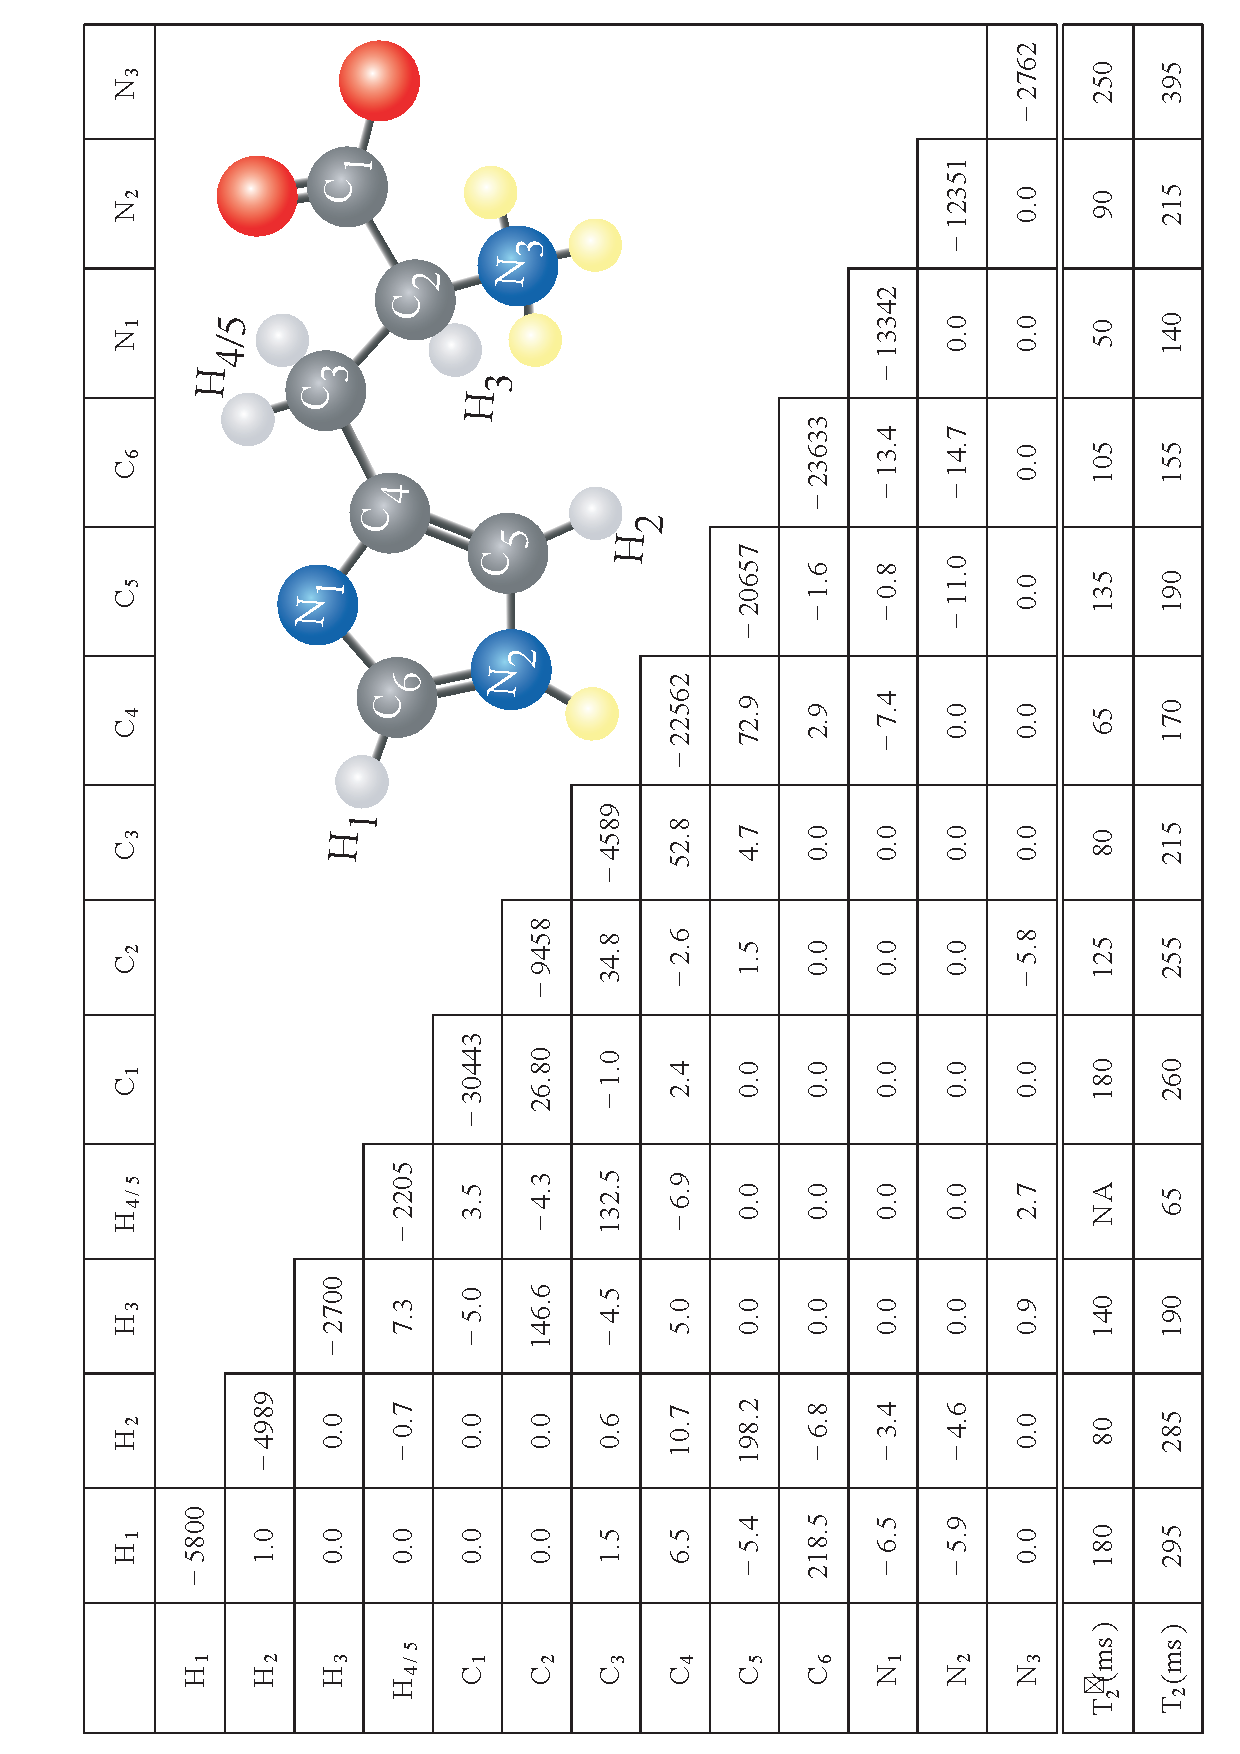
\includegraphics[width= 0.8\columnwidth]{figures/samplemost.pdf}
              \caption{12 qubit \emph{l}-Histidine的分子结构及参数大小。H4和H5可以当做一个自旋为1的粒子来处理。}
              \label{samplemost}
            \end{center}
\end{figure}